\chapter{Adversarial evaluation}\label{ch:adv_eval}

\par In this part, I mention an experiment I performed, in order to investigate the problem of using an oracle to evaluate the generator, and use the quality assessment of the oracle as a feedback to the generator, in order to improve it. I will first describe what is the problem, then explain the hypothesis, and then show the experiments performed, and the lessons learned.

\par A similar work was done in~\citep{nguyen2015deep} \footnote{I was not aware of that work beforehand. The paper is neatly explained though.} and heavily inspired by the work done in~\citep{adv_attack_presentation}. I would like to thank \textit{Ludovic Darmet} for the valuable discussions and resources about this topic.

\section{What is the problem?\footnote{The images in this section are taken from~\citep{adv_attack_presentation}.}}
  \par Given a data distribution that separates points into two classes (as in figure~\ref{fig:gen_er1}), and given some examples from that distribution (the sampled data points), the objective is to estimate this decision boundary given the sampled data points, figure~\ref{fig:gen_er2}. Using test data in order to estimate the errors of the model estimation does not always reveal the problem or the boundaries that the model actually learned, figure~\ref{fig:gen_er3}.

  \par This is where adversarial examples comes in. Adversarial examples exploit the fact that that the there is a difference between the ground truth decision boundary and the model approximated decision boundary. The model is blind about what the reality looks like, thus, it can be exploited by some fake examples, in order to generate improper classification, figure~\ref{fig:gen_er4}. The problem gets worse when we increase dimensionality of the problem -- \textit{curse of dimensionality} --.
  \begin{figure}
    \centering
    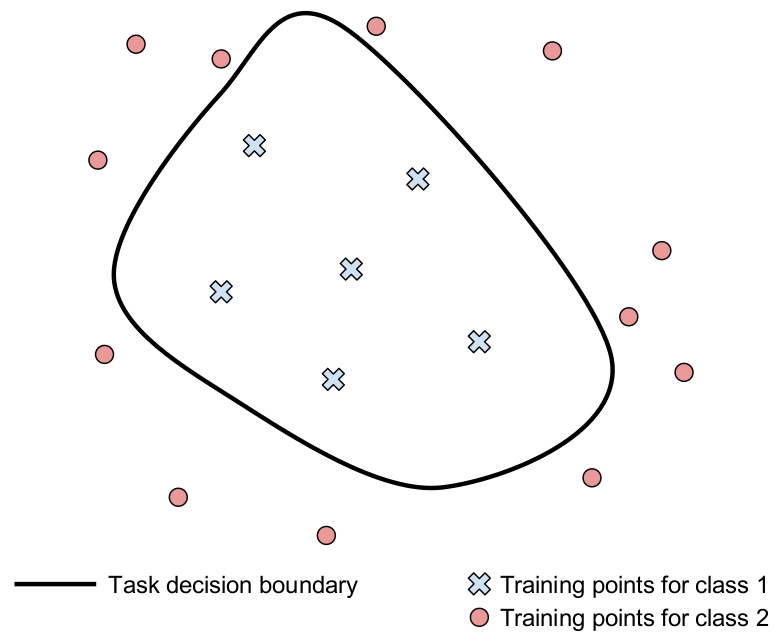
\includegraphics[scale=0.3]{images/adv_attack/gen_er1.png}
    \caption{The ground truth decision boundary that separates data into two classes. This decision boundary is unknown in advance. The objective of machine learning is to estimate/approximate/learn this decision boundary.}
    \label{fig:gen_er1}
  \end{figure}

  \begin{figure}
    \centering
    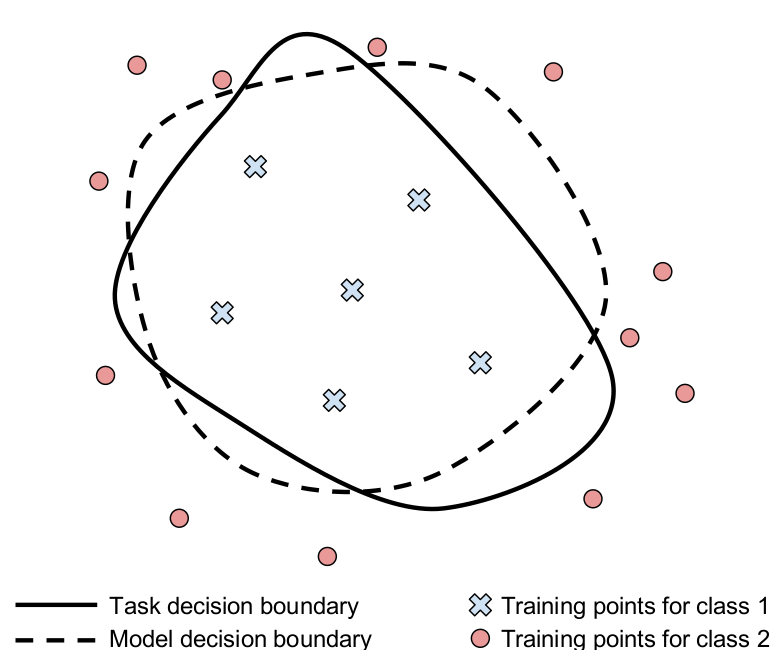
\includegraphics[scale=0.3]{images/adv_attack/gen_er2.png}
    \caption{The machine learning model estimate the decisions boundary based on the given examples. The estimation is not perfect, and not necessarily matches the ground truth boundary.}
    \label{fig:gen_er2}
  \end{figure}

  \begin{figure}
    \centering
    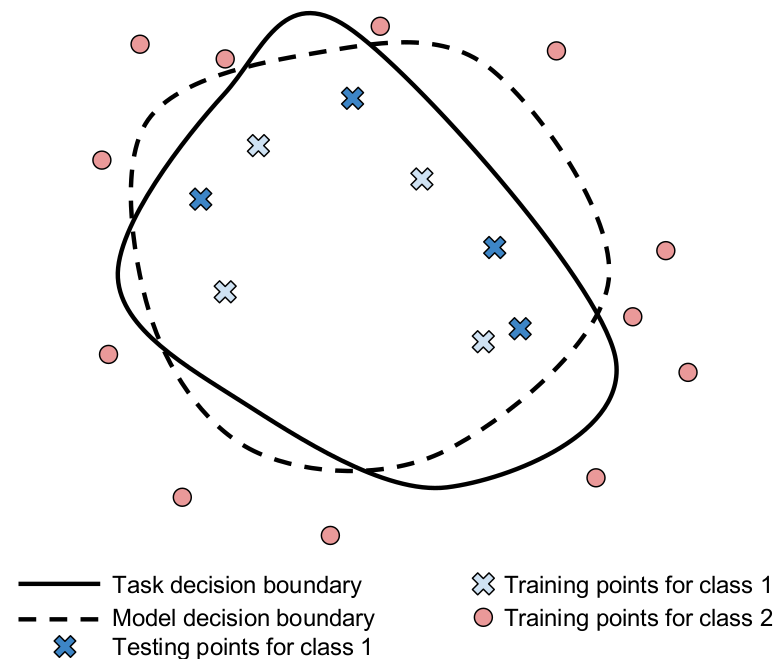
\includegraphics[scale=0.3]{images/adv_attack/gen_er3.png}
    \caption{Using the test data, sometimes we do not get a sense for the limitations of the model approximation. Even when the model shows errors, it is not possible to estimate the boundaries of the model approximation from this information.}
    \label{fig:gen_er3}
  \end{figure}

  \begin{figure}
    \centering
    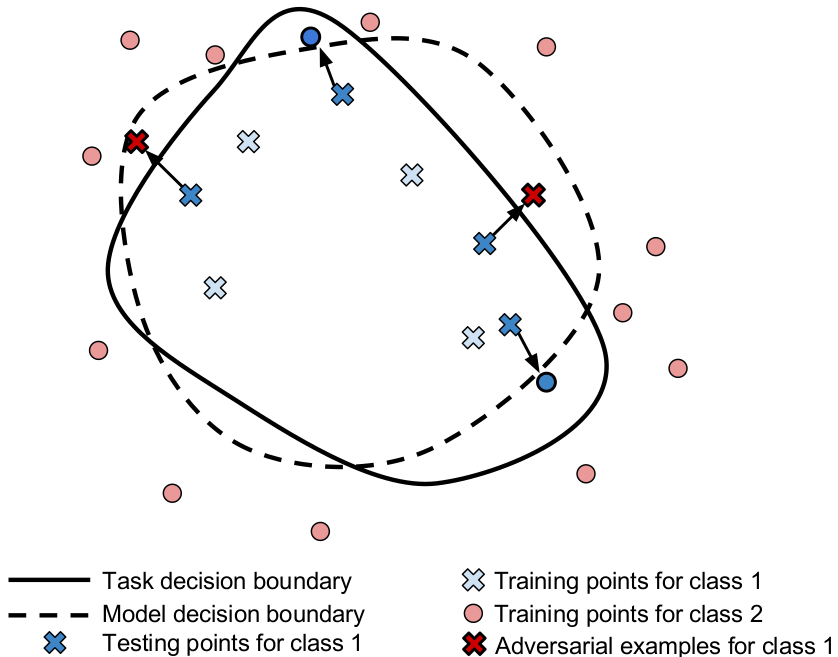
\includegraphics[scale=0.3]{images/adv_attack/gen_er4.png}
    \caption{Adversarial examples exploit the fact that the model only approximates the ground truth decision boundary, thus, there is a gap between them. Using this gap can easily misguide the model and lead to misclassification.}
    \label{fig:gen_er4}
  \end{figure}

\section{How to test this?}
  \par I designed an experiment in order to see how this actually works. I build a variety of classifier models (oracles) -- in order study the phenomena across multiple algorithms -- on the MNIST dataset~\citep{lecun-mnisthandwrittendigit-2010}, figure~\ref{fig:mnist}, and then build an image generator that is optimized on the outcome of each classifier. The optimizer is an genetic algorithm~\citep{eiben2003introduction}. The experiment setup is shown in figure~\ref{fig:adversarial_exp_setup}. Different algorithms had been tested, starting from logistic regression, kNN, neural networks and random forests.

  \begin{figure}
    \centering
    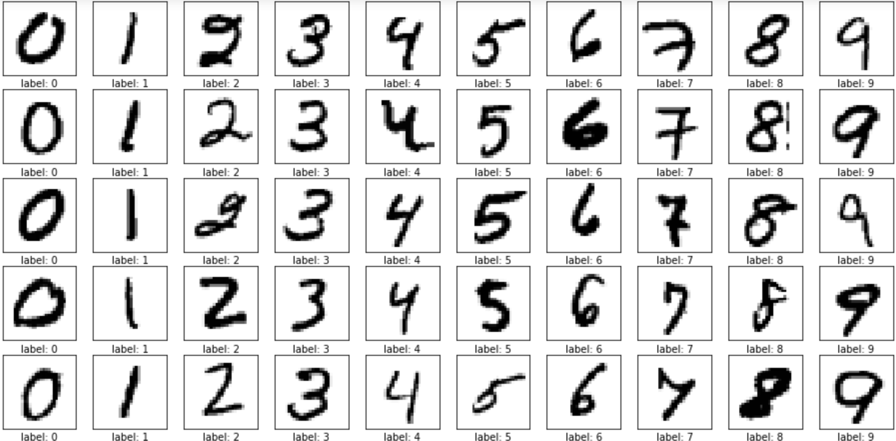
\includegraphics[scale=0.4]{images/adv_attack/mnist.png}
    \caption{MNIST is a popular offline handwriting dataset for digits from 0-9. 70K examples are available, 60K for training/validation and 10K for testing. The images size is 64x64.}
    \label{fig:mnist}
  \end{figure}

  \begin{figure}
    \centering
    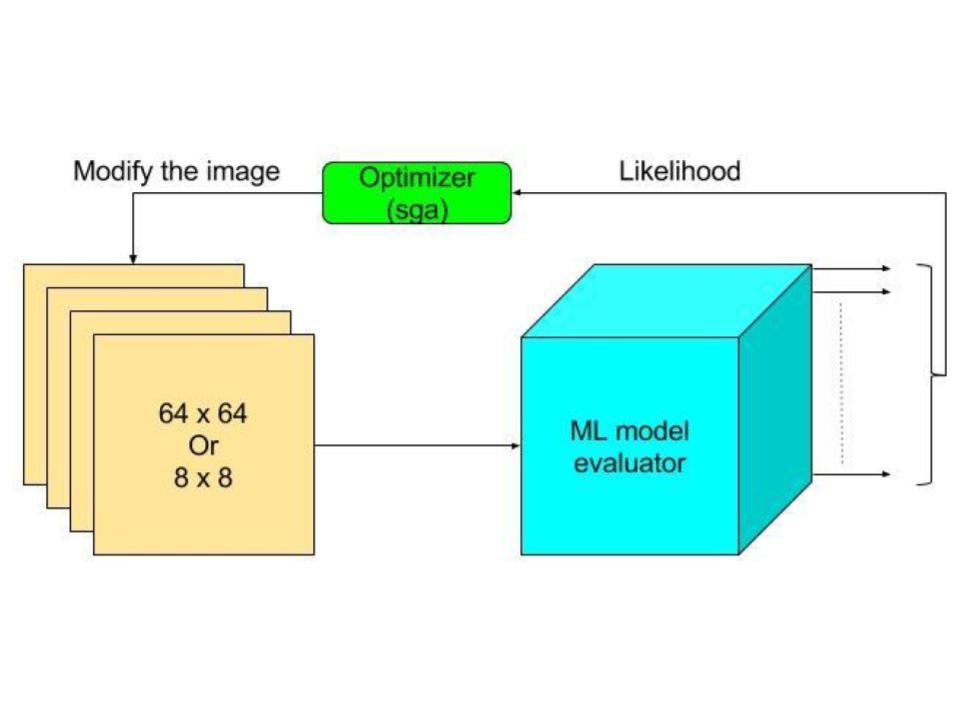
\includegraphics[scale=0.4]{images/adv_attack/adversarial_optimization.png}
    \caption{The setup of the experiment to understand the effect of using an oracle as the guidance for training a generator. The oracles were trained on MNIST dataset in order to classify the digits, and the generator is optimized based on what the oracle output. The generator objective is to generate images for different digits.}
    \label{fig:adversarial_exp_setup}
  \end{figure}

\section{What is the lesson learned?}
  \par Even if the model (oracle) is doing extremely well on the ground-truth distribution, it is should not be used naively as a replacement for the ground truth, in order to evaluate other models (like a generator). The generator can easily learn how to deceives the oracle in order to maximize the final performance numbers, without any consideration for what these numbers implies. I believe that this is an interesting direction in research though, with a lot of potential, by developing some safeguards to protect the model from being deceived, reporting the model confidence about the current input, or having some estimation for the model error once we change the distribution.
